%%%%%%%%%%%%%%%%%%%%%%%%%%%%%%%%%%%%%%%%%
% Beamer Presentation
% LaTeX Template
% Version 1.0 (10/11/12)
%
% This template has been downloaded from:
% http://www.LaTeXTemplates.com
%
% License:
% CC BY-NC-SA 3.0 (http://creativecommons.org/licenses/by-nc-sa/3.0/)
%
%%%%%%%%%%%%%%%%%%%%%%%%%%%%%%%%%%%%%%%%%

%----------------------------------------------------------------------------------------
%	PACKAGES AND THEMES
%----------------------------------------------------------------------------------------

\documentclass{beamer}

\mode<presentation> {

% The Beamer class comes with a number of default slide themes
% which change the colors and layouts of slides. Below this is a list
% of all the themes, uncomment each in turn to see what they look like.

%\usetheme{default}
%\usetheme{AnnArbor}
%\usetheme{Antibes}
%\usetheme{Bergen}
%\usetheme{Berkeley}
\usetheme{Berlin}
%\usetheme{Boadilla}
%\usetheme{CambridgeUS}
%\usetheme{Copenhagen}
%\usetheme{Darmstadt}
%\usetheme{Dresden}
%\usetheme{Frankfurt}
%\usetheme{Goettingen}
%\usetheme{Hannover}
%\usetheme{Ilmenau}
%\usetheme{JuanLesPins}
%\usetheme{Luebeck}
%\usetheme{Madrid}
%\usetheme{Malmoe}
%\usetheme{Marburg}
%\usetheme{Montpellier}
%\usetheme{PaloAlto}
%\usetheme{Pittsburgh}
%\usetheme{Rochester}
%\usetheme{Singapore}
%\usetheme{Szeged}
%\usetheme{Warsaw}

% As well as themes, the Beamer class has a number of color themes
% for any slide theme. Uncomment each of these in turn to see how it
% changes the colors of your current slide theme.

%\usecolortheme{albatross}
%\usecolortheme{beaver}
%\usecolortheme{beetle}
%\usecolortheme{crane}
%\usecolortheme{dolphin}
%\usecolortheme{dove}
%\usecolortheme{fly}
%\usecolortheme{lily}
%\usecolortheme{orchid}
%\usecolortheme{rose}
%\usecolortheme{seagull}
%\usecolortheme{seahorse}
%\usecolortheme{whale}
%\usecolortheme{wolverine}

%\setbeamertemplate{footline} % To remove the footer line in all slides uncomment this line
%\setbeamertemplate{footline}[page number] % To replace the footer line in all slides with a simple slide count uncomment this line

%\setbeamertemplate{navigation symbols}{} % To remove the navigation symbols from the bottom of all slides uncomment this line
}

\usepackage{graphicx} % Allows including images
\usepackage{booktabs} % Allows the use of \toprule, \midrule and \bottomrule in tables
%\usepackage[brazilian]{babel}
\usepackage[utf8]{inputenc}
\usepackage{listings}
\usepackage{amsmath}
\usepackage{amsfonts}
\usepackage{pdfpages}
\usepackage{textpos}

\graphicspath{ {img/} }

%----------------------------------------------------------------------------------------
%	TITLE PAGE
%----------------------------------------------------------------------------------------

\title[Generating Acrostics via Paraphrasing and Heuristic Search]{Generating Acrostics via Paraphrasing and Heuristic Search} % The short title appears at the bottom of every slide, the full title is only on the title page

\author[Bruno, Fernando, Jürgen, William]{Bruno Soares Fillmann\\
Fernando Bombardelli da Silva\\
Jürgen Bauer\\
William Bombardelli da Silva
} % Your name
\institute[TU Berlin] % Your institution as it will appear on the bottom of every slide, may be shorthand to save space
{
Technische Universität Berlin \\ % Your institution for the title page
Datenbanksysteme und Informationsmanagement \\
DBPRO – Database Projects (WS 2014/2015) \\
\medskip
%\textit{fbdasilva@inf.ufrgs.br} % Your email address
}
\date{12.01.2015} % Date, can be changed to a custom date

\begin{document}

\begin{frame}
\titlepage % Print the title page as the first slide
\end{frame}

\begin{frame}
\frametitle{Organization} % Table of contents slide, comment this block out to remove it
\tableofcontents % Throughout your presentation, if you choose to use \section{} and \subsection{} commands, these will automatically be printed on this slide as an overview of your presentation
\end{frame}

%----------------------------------------------------------------------------------------
%	PRESENTATION SLIDES
%----------------------------------------------------------------------------------------

%------------------------------------------------
\section{Overview} % Sections can be created in order to organize your presentation into discrete blocks, all sections and subsections are automatically printed in the table of contents as an overview of the talk
%------------------------------------------------

%\subsection{Subsection Example} % A subsection can be created just before a set of slides with a common theme to further break down your presentation into chunks

\begin{frame}
\frametitle{Overview}
\begin{itemize}
\item \textbf{The problem:} Given a text T and an acrostic X, find a paraphrased version of T that encodes X in the first letters of each line.
\item \textbf{Main goal of the project:} Implement the paper for the German language.
\item \textbf{Main idea of the algorithm:}
	\begin{itemize}
	\item Modeled as a search problem in a tree.
	\item The vertices are states (texts) and the edges are operations over states.
	\item Artificial intelligence is applied for the search strategy (A* Algorithm).
	\end{itemize}
\end{itemize}
\end{frame}

%------------------------------------------------
\section{New Operations}
%------------------------------------------------
\begin{frame}
\frametitle{Hyphenation}


\begin{itemize}
\item Line Length constraints $l_{min}=50$ and $l_{max}=70.$



\item For hyphenation a re-implementation of Knuth's hyphenation algorithm in
TeX is used (TEXHyphenator-J by David Tolpin) 

\item A word can be hyphenated if: The part of the current line \textbf{up to} the hyphen has a length of at least $l_{min}=50.$

\item The text \textbf{after} the hyphen has to be aligned again to fulfill the line length
constraints.



\item A greedy word wrap algorithm is applied. 

\item Don't allow words of length $>20$ in the start text.
\end{itemize}

\end{frame}



\begin{frame}
\frametitle{Hyphenation}

%\begin{textblock}{200}(0,0)
%\leavevmode
%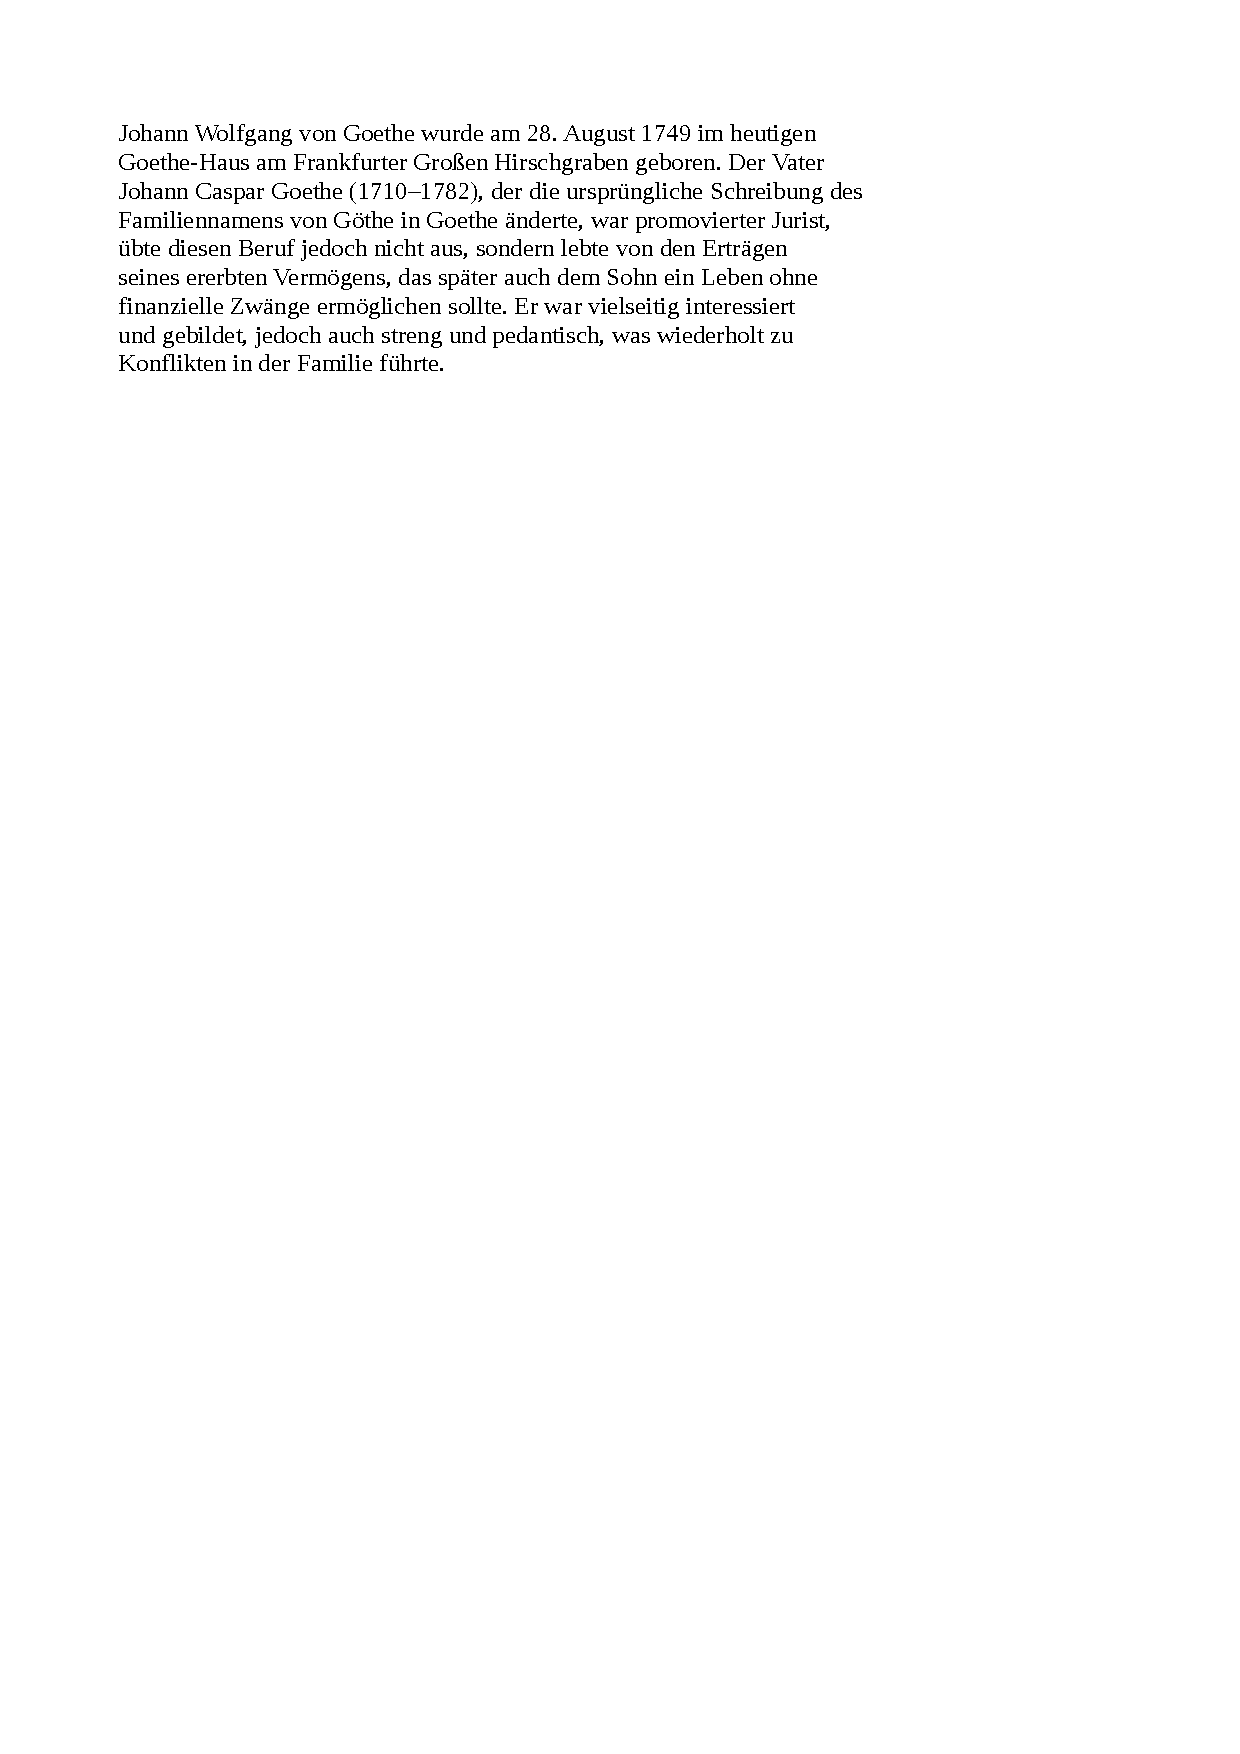
\includegraphics[scale=0.5]{Goethe.pdf}

%\put(0,50){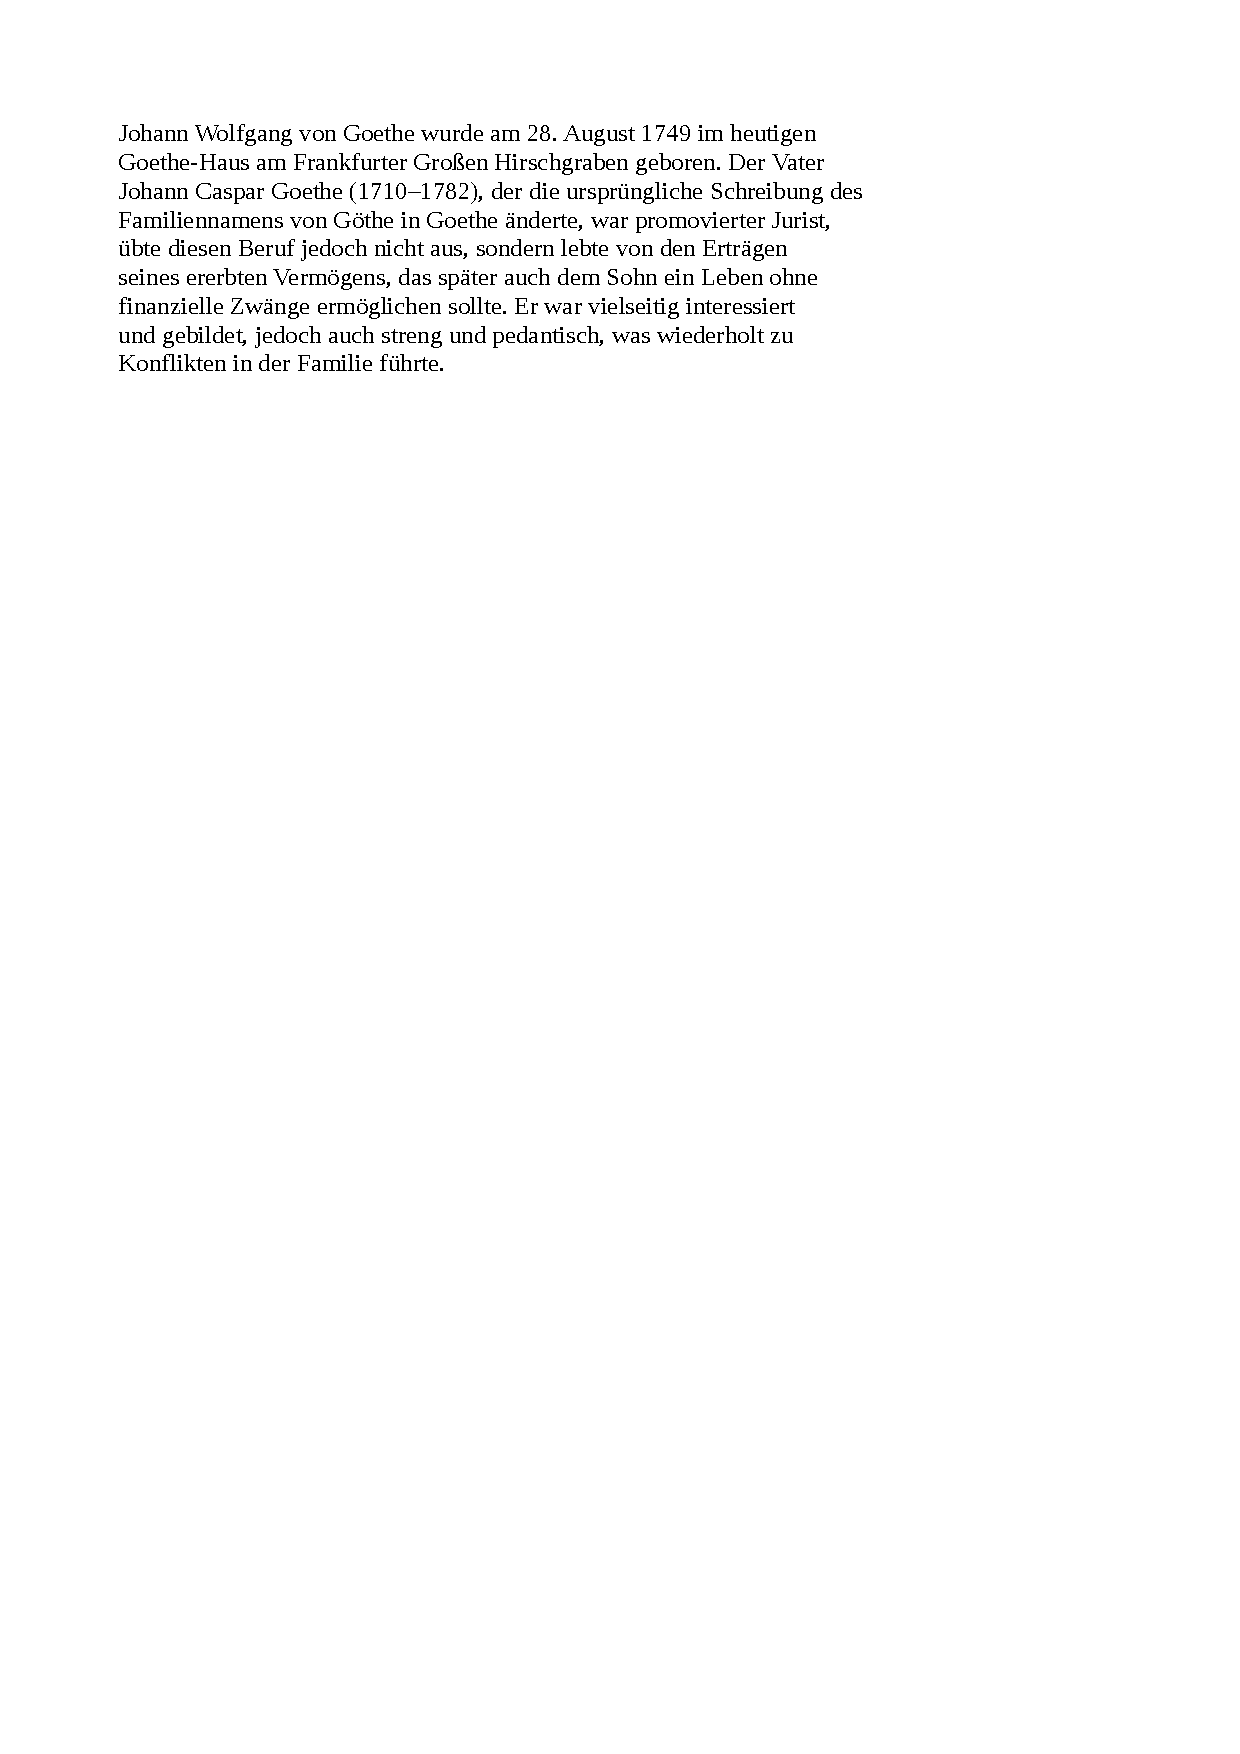
\includegraphics[scale=0.5]{Goethe.pdf}}
%\end{textblock}

\begin{itemize}
%\item \textbf{Example:}

\item \textbf{Example:}
\item 38 hyphenations!
%\item Hier steht ein längerer Text mit Foto
%\end{itemize}

\end{itemize}

\begin{picture}(300,400)
\put(-10,-165){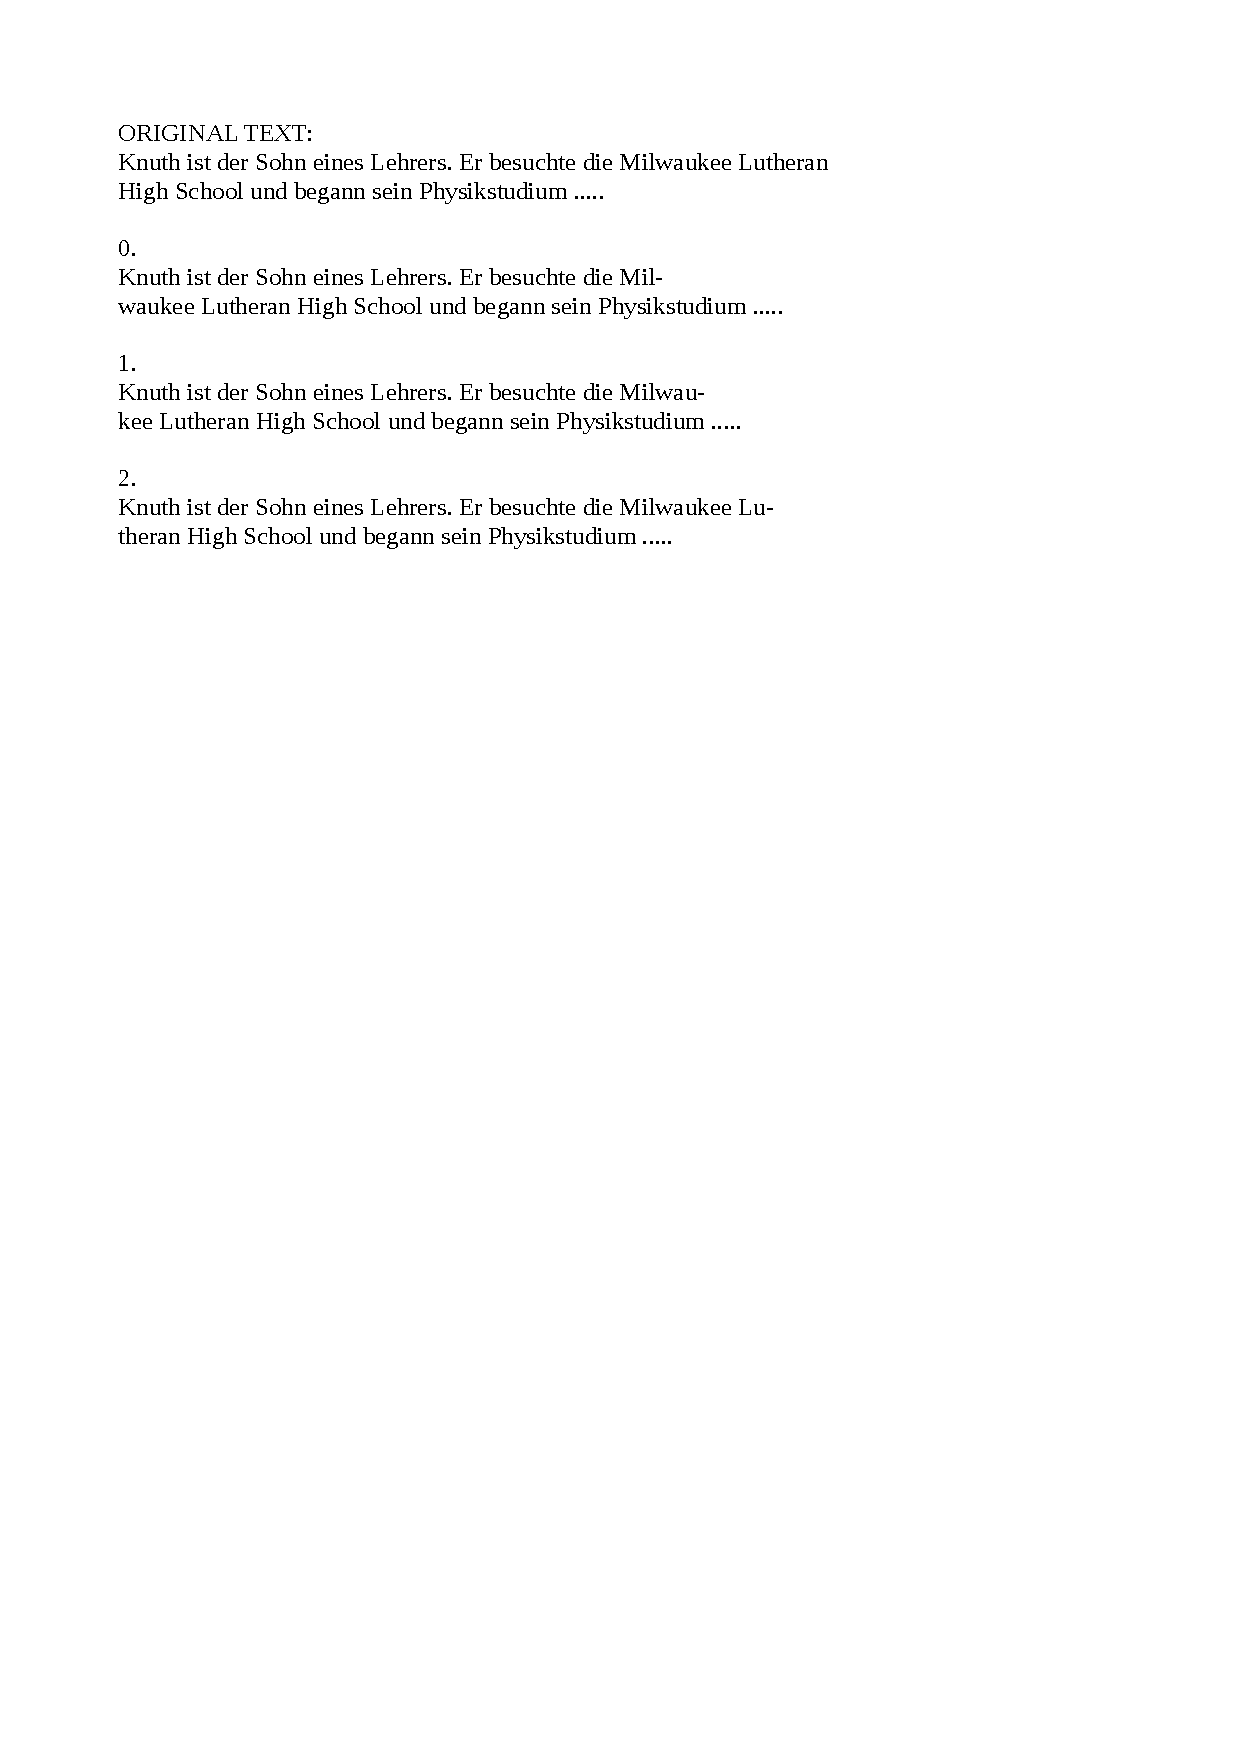
\includegraphics[scale=0.7]{KnuthHyphenation.pdf}}
\end{picture}





%\begin{picture}(220,450)
%\put(40,80){ 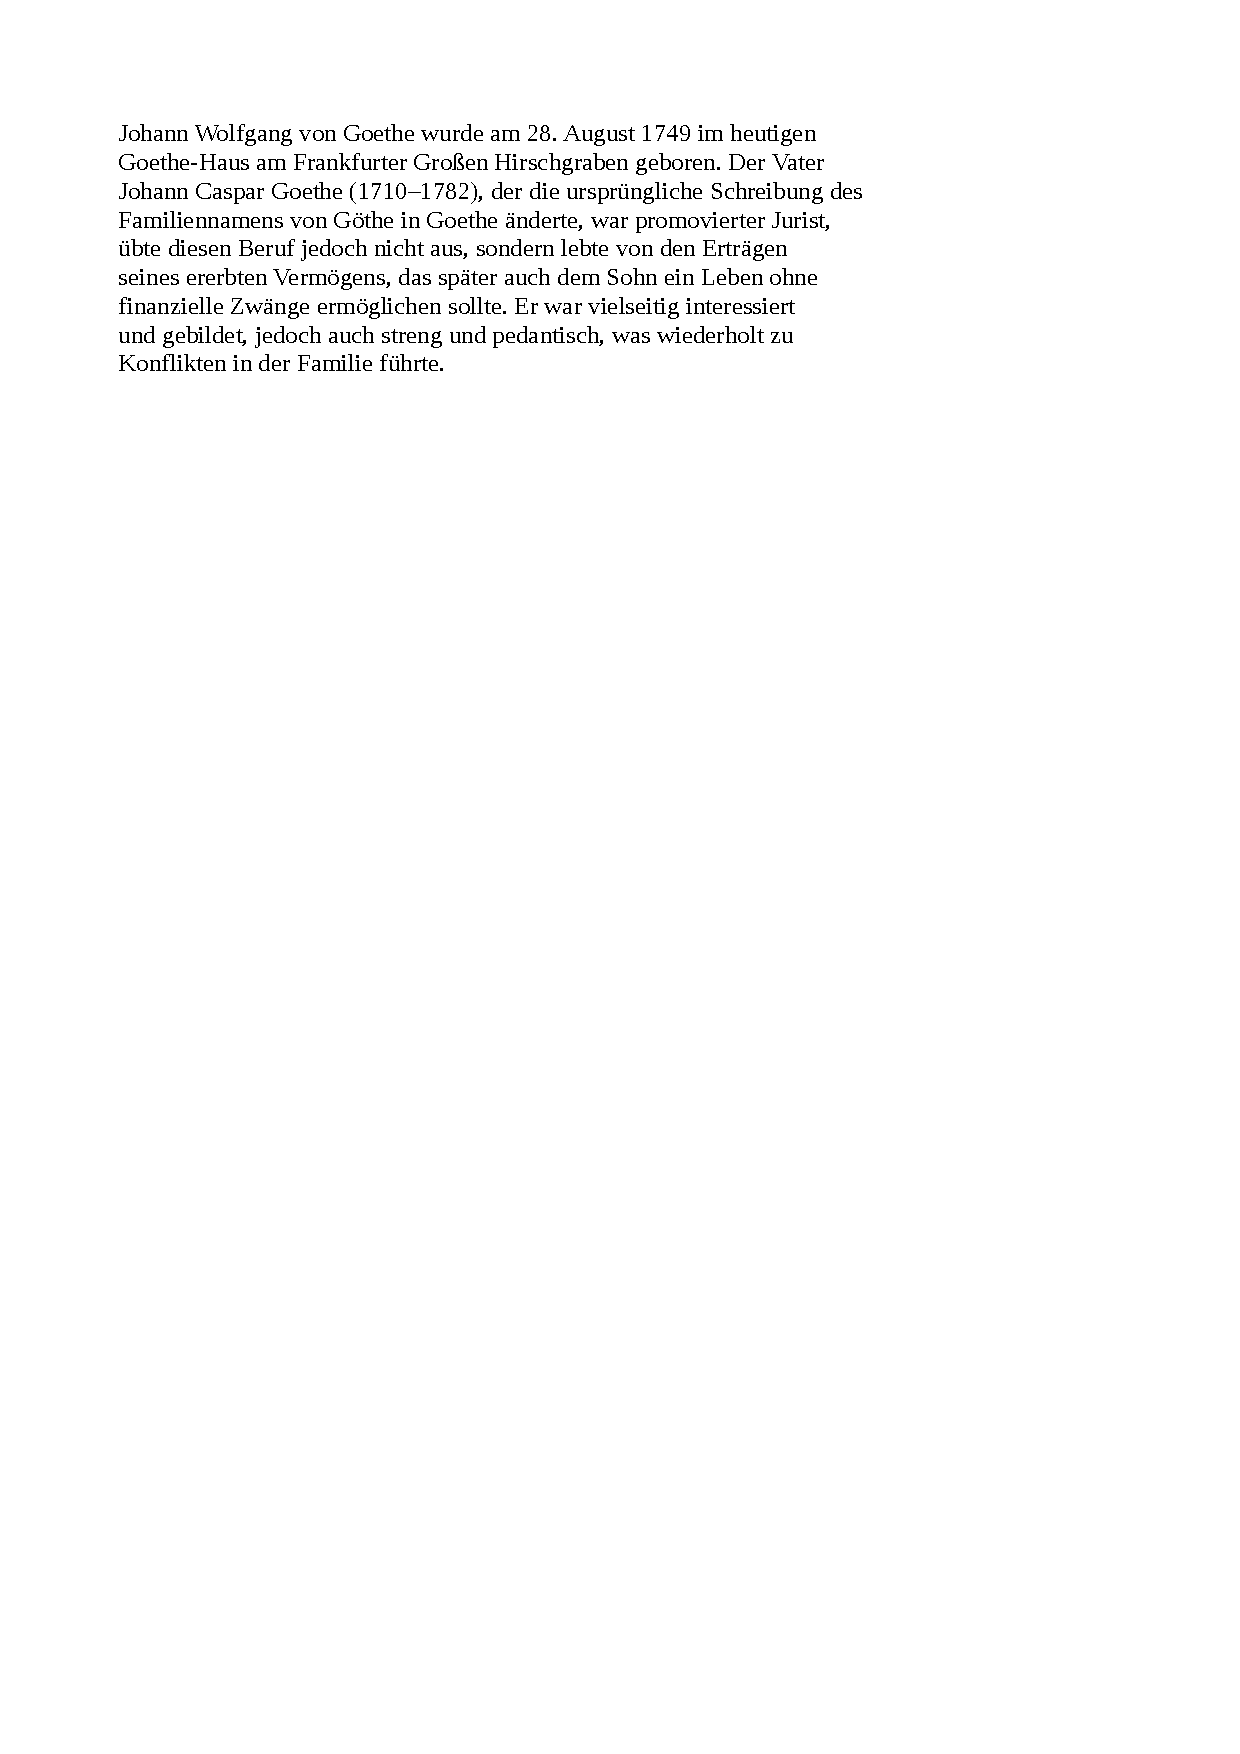
\includegraphics[height=15\textheight]{Goethe.pdf} }
%\end{picture}



\end{frame}


\begin{frame}
\frametitle{Examples}

%\begin{textblock}{200}(0,0)
%\leavevmode
%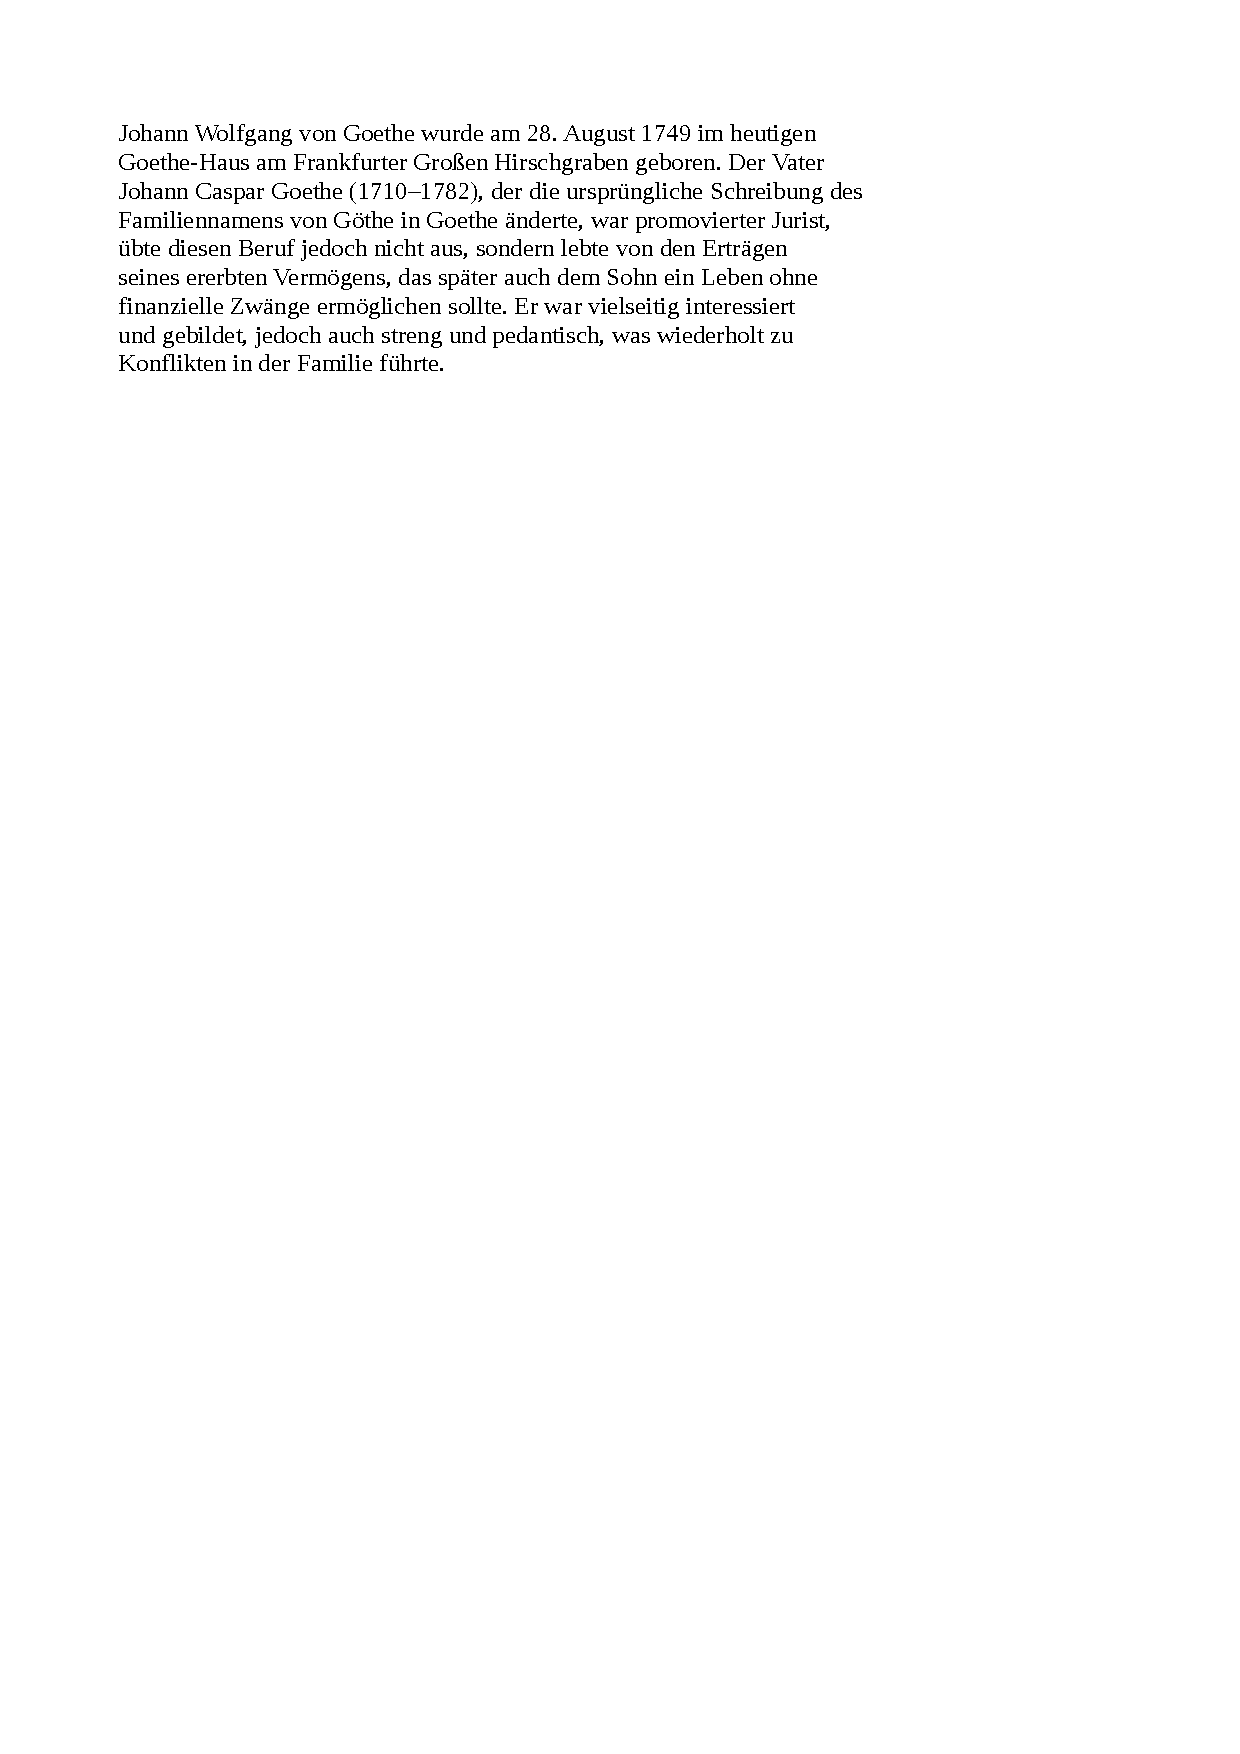
\includegraphics[scale=0.5]{Goethe.pdf}

%\put(0,50){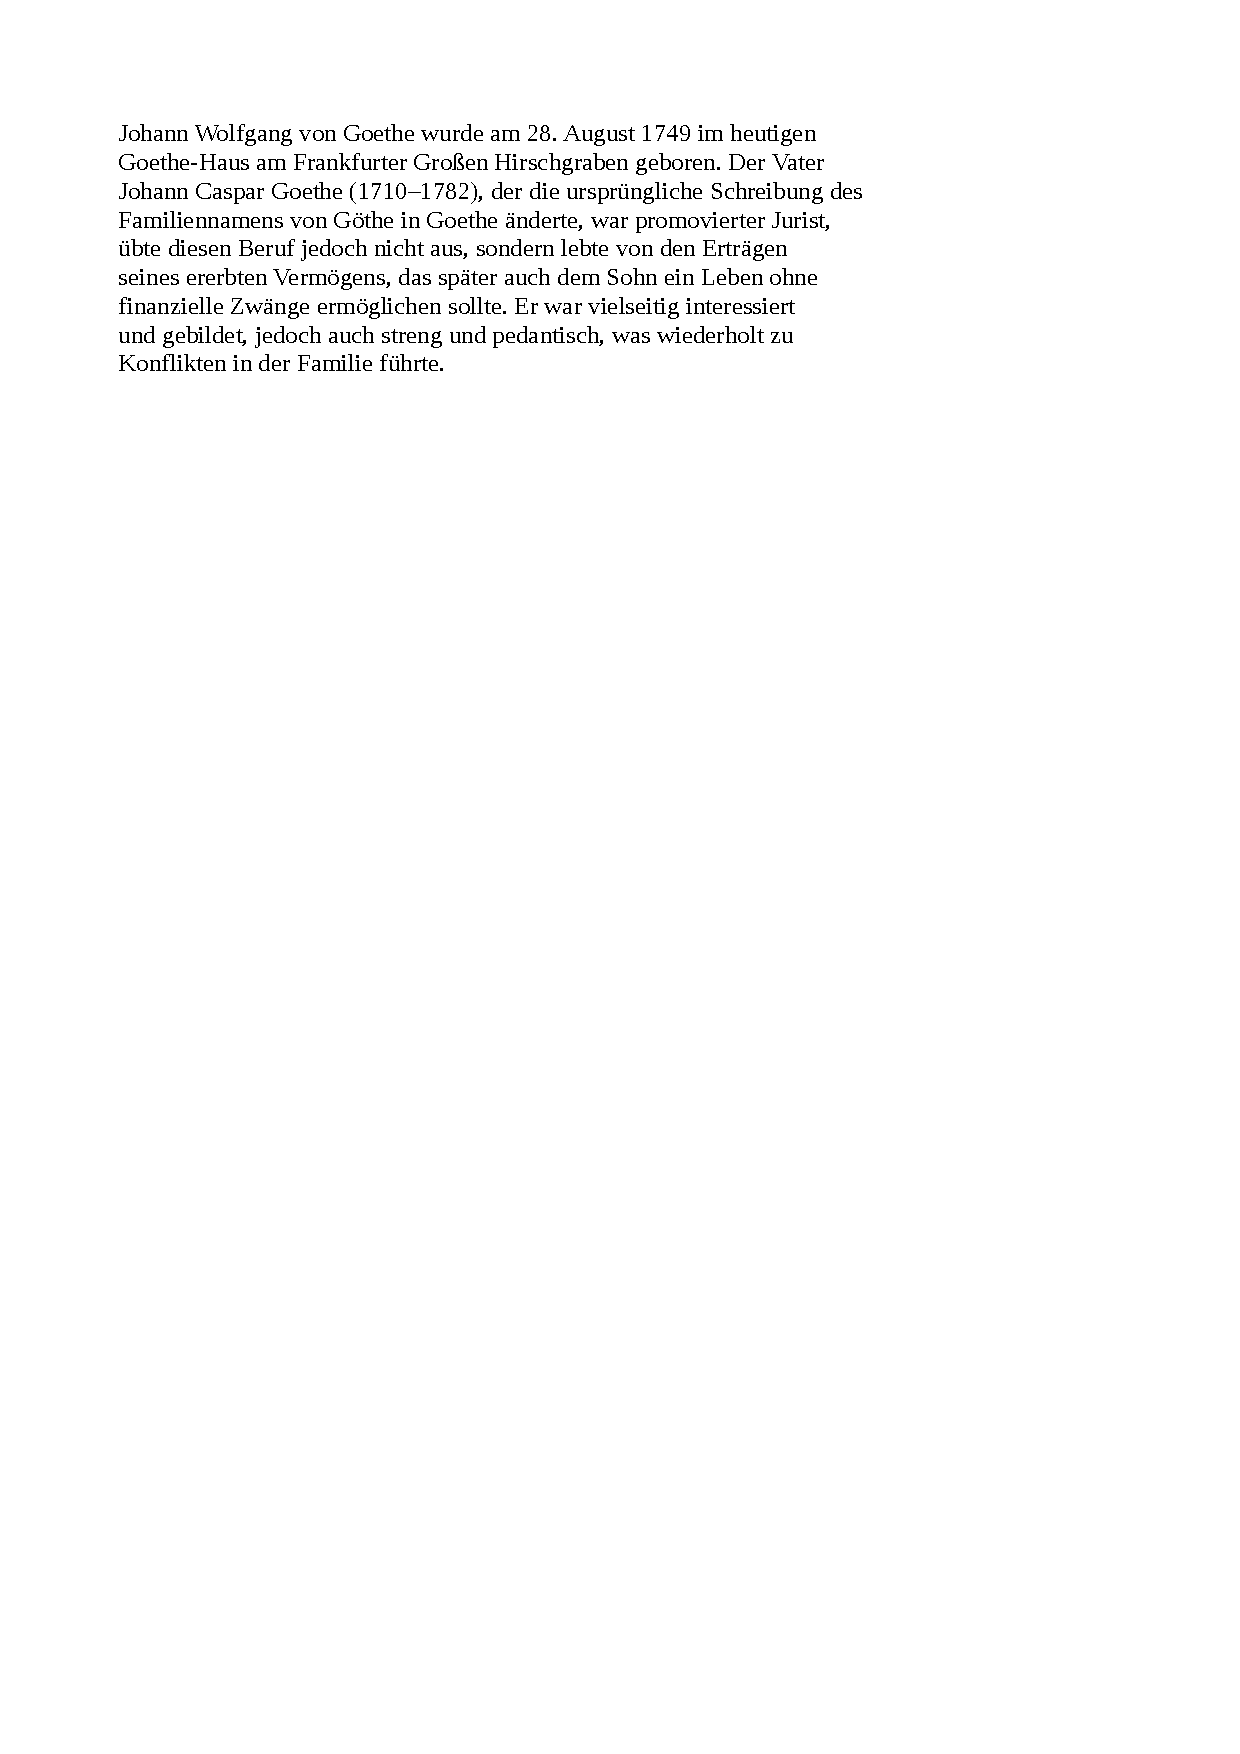
\includegraphics[scale=0.5]{Goethe.pdf}}
%\end{textblock}

\begin{itemize}
%\item \textbf{Example:}


\item  1 min 22 sec, 17517 nodes, Ops: Hyph,WrHyph,LB
%\item Hier steht ein längerer Text mit Foto
%\end{itemize}

\end{itemize}

\begin{picture}(300,400)
\put(-10,-165){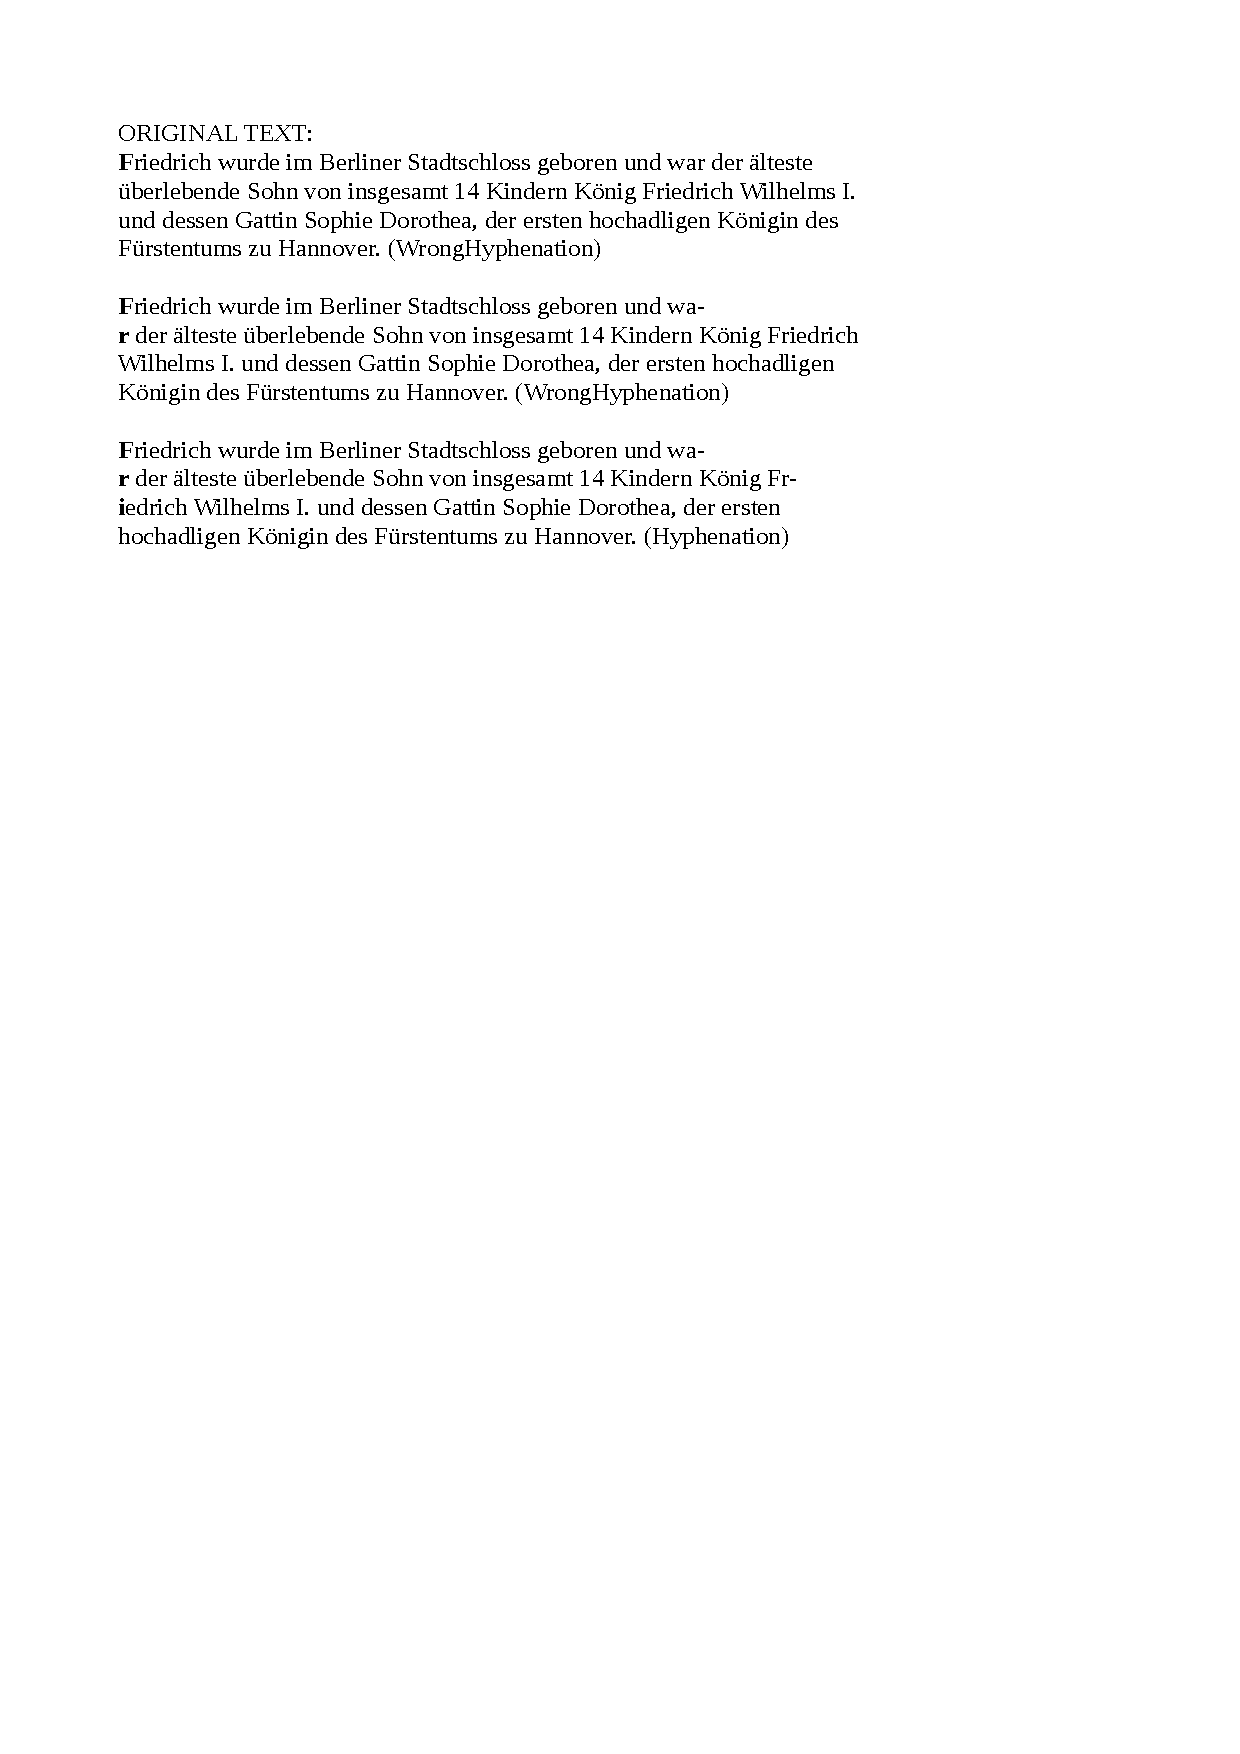
\includegraphics[scale=0.7]{FritzExample.pdf}}
\end{picture}





%\begin{picture}(220,450)
%\put(40,80){ 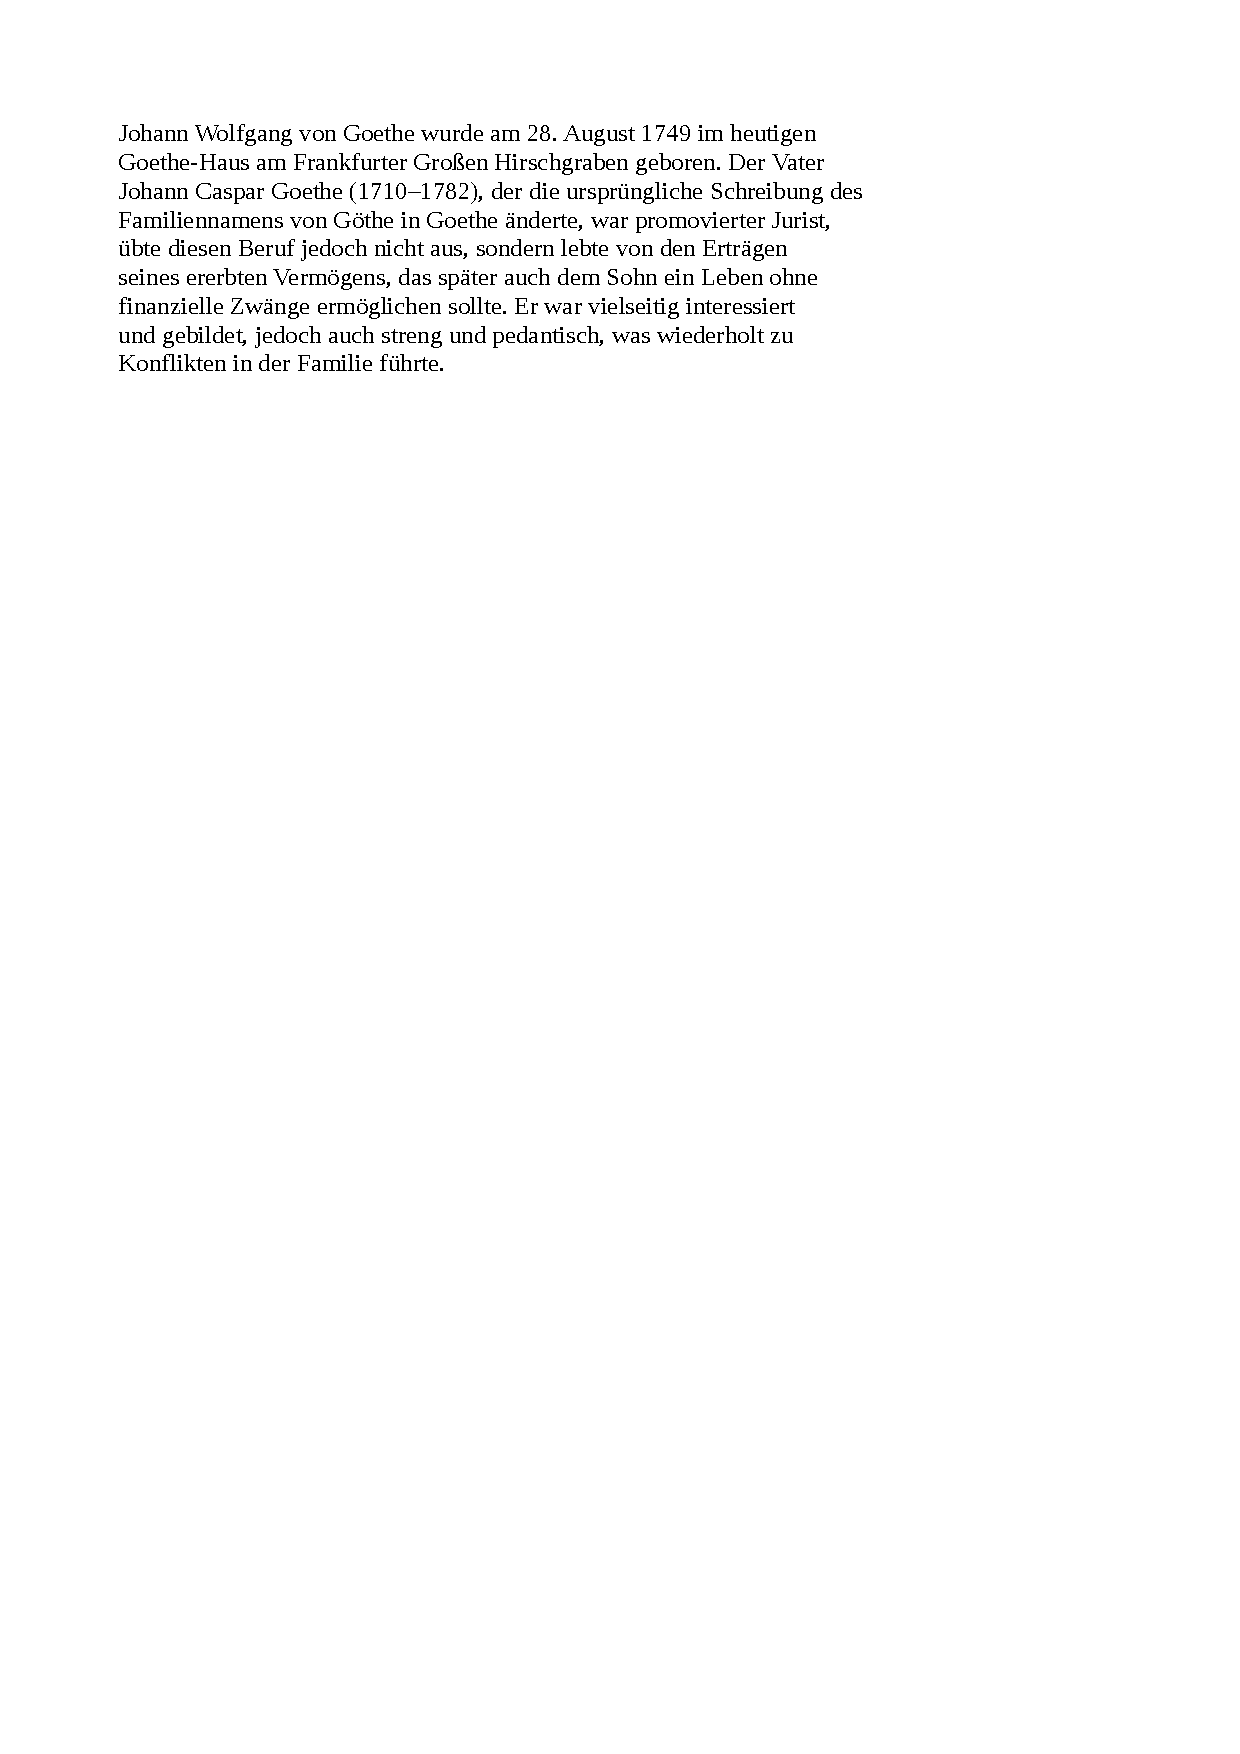
\includegraphics[height=15\textheight]{Goethe.pdf} }
%\end{picture}



\end{frame}



\begin{frame}
\frametitle{Examples}

%\begin{textblock}{200}(0,0)
%\leavevmode
%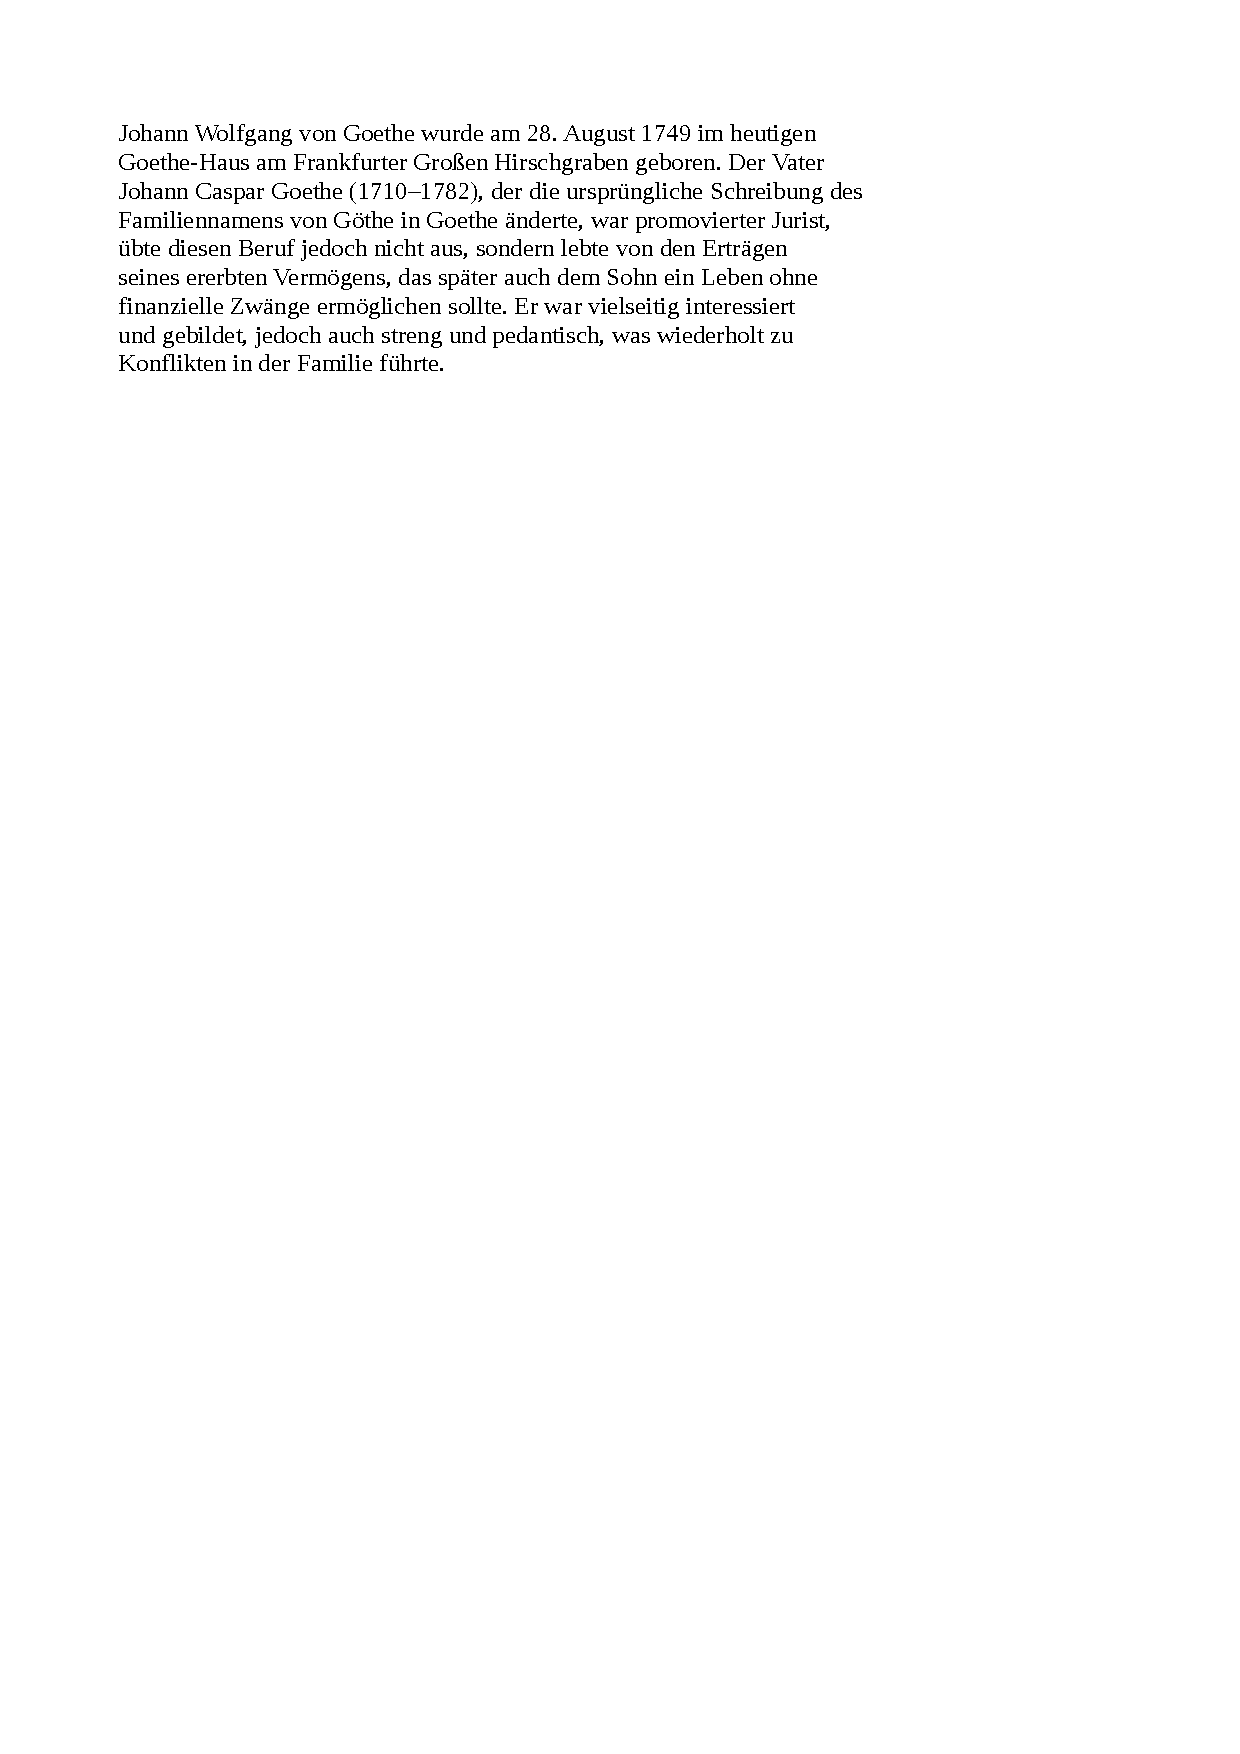
\includegraphics[scale=0.5]{Goethe.pdf}

%\put(0,50){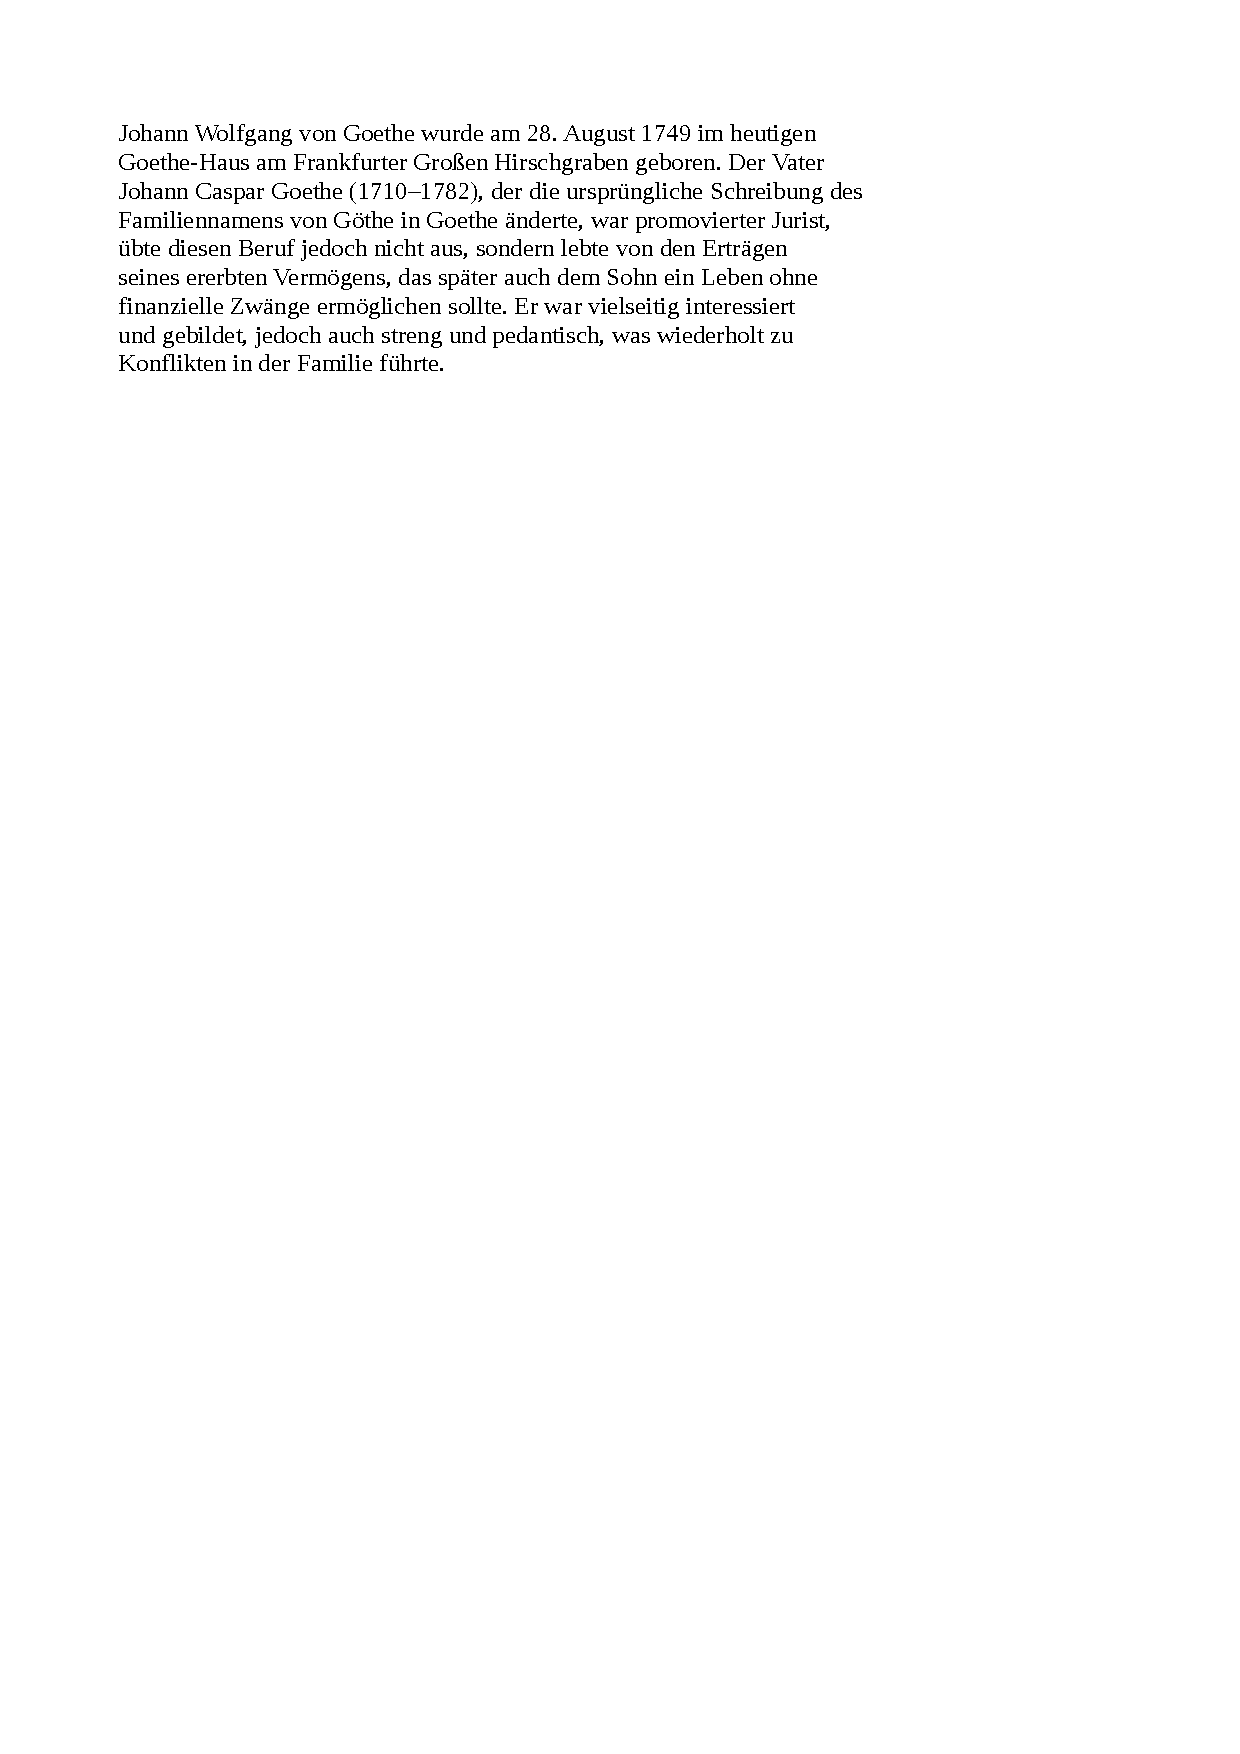
\includegraphics[scale=0.5]{Goethe.pdf}}
%\end{textblock}

\begin{itemize}
%\item \textbf{Example:}


\item  1 min 22 sec, 17517 nodes, Ops: Hyph,WrHyph,LB
%\item Hier steht ein längerer Text mit Foto
%\end{itemize}

\end{itemize}

\begin{picture}(300,400)
\put(-10,-165){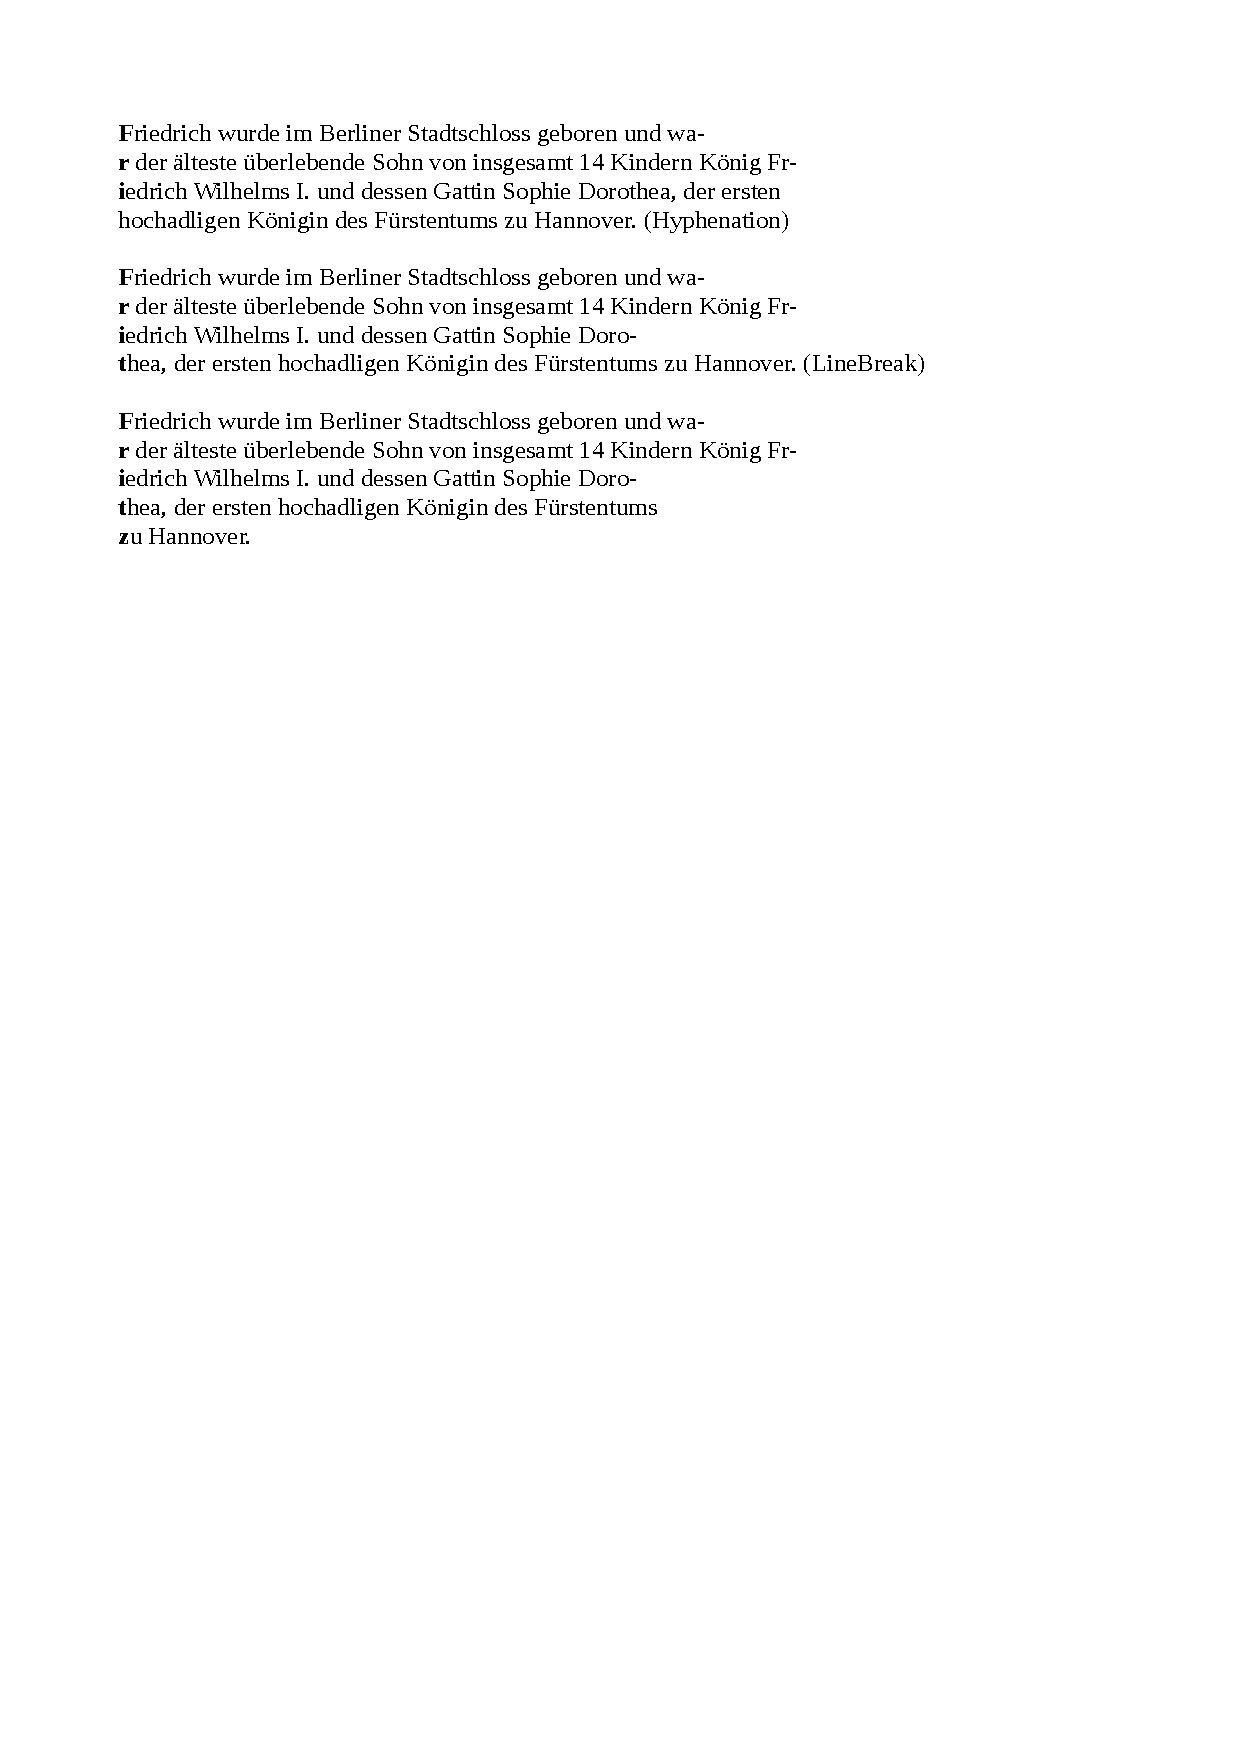
\includegraphics[scale=0.7]{FritzExample2.pdf}}
\end{picture}





%\begin{picture}(220,450)
%\put(40,80){ 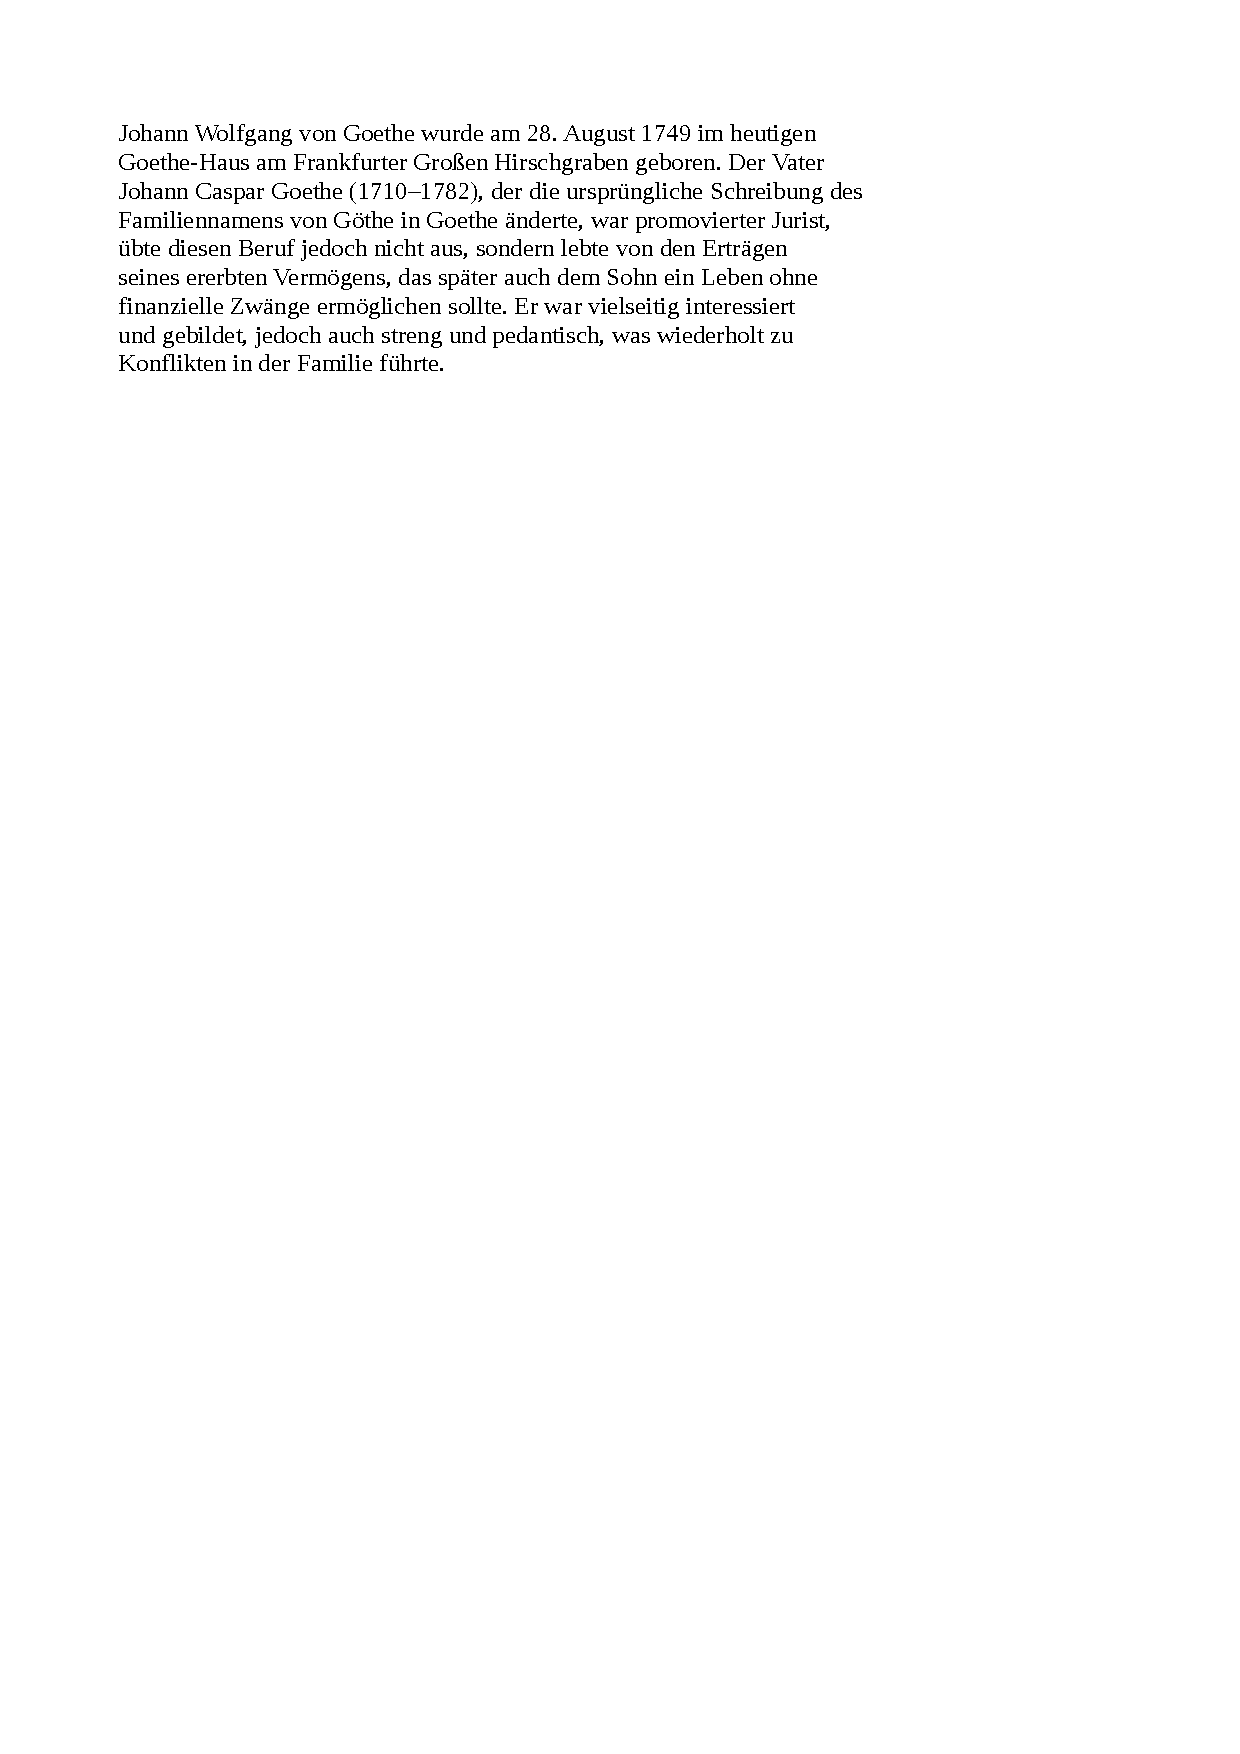
\includegraphics[height=15\textheight]{Goethe.pdf} }
%\end{picture}



\end{frame}















%------------------------------------------------
\section{New Results}
%------------------------------------------------

\begin{frame}
\frametitle{First Results $-$ Goethe}
\texttt{\tiny
Johann Wolfgang von Goethe wurde am 28. August 1749 im heutigen \\
Goethe-Haus am Frankfurter Großen Hirschgraben geboren. Der Vater \\
Johann Caspar Goethe (1710–1782), der die ursprüngliche Schreibung des \\
Familiennamens von Göthe in Goethe änderte, war promovierter Jurist, \\
übte diesen Beruf jedoch nicht aus, sondern lebte von den Erträgen \\
seines ererbten Vermögens, das später auch dem Sohn ein Leben ohne \\
finanzielle Zwänge ermöglichen sollte. Er war vielseitig interessiert \\
und gebildet, jedoch auch streng und pedantisch, was wiederholt zu \\
Konflikten in der Familie führte. \\
}

Result Text: \\

\texttt{\scriptsize{J}\tiny ohann Wolfgang von Goethe wurde am 28. August 1749 im he- \hskip 16pt \emph{//Wrong Hyphenation} \\
\scriptsize{u}\tiny tigen Goethe-Haus am Frankfurter Großen Hirschgraben gebore- \hskip 10pt \emph{//LineBreak + Wrong Hyphenation} \\
\scriptsize{n}\tiny . Der Vater Johann Caspar Goethe (1710–1782), der die ursprün- \emph{//Wrong Hyphenation} \\
\scriptsize{g}\tiny liche Schreibung des Familiennamens von Göthe in Goethe änderte, war \\
promovierter Jurist, übte diesen Beruf jedoch nicht aus, sondern lebte \\
von den Erträgen seines ererbten Vermögens, das später auch dem Sohn \\
ein Leben ohne finanzielle Zwänge ermöglichen sollte. Er war \\
vielseitig interessiert und gebildet, jedoch auch streng und \\
pedantisch, was wiederholt zu Konflikten in der Familie führte. \\
}
\end{frame}

%------------------------------------------------
\section{Conclusion}
%------------------------------------------------

\begin{frame}
\frametitle{Conclusion}
\begin{itemize}
\item bla blah blah
\end{itemize}
\end{frame}

%------------------------------------------------
\section{References}
%------------------------------------------------

\begin{frame}
\frametitle{References}
\footnotesize
\begin{thebibliography}{1}
\bibitem{Stein}
	Benno Stein, Matthias Hagen, and Christof Bräutigam. \emph{Generating Acrostics via Paraphrasing and Heuristic Search}. \\
	In Junichi Tsujii and Jan Hajic, editors, 25th International Conference on Computational Linguistics (COLING 14), pages 2018-2029, August 2014. Association for Computational Linguistics.
\end{thebibliography}
\end{frame}
%------------------------------------------------

\begin{frame}
\Huge{\centerline{Questions?}}
\end{frame}

%----------------------------------------------------------------------------------------

\end{document}
